\documentclass[12pt]{article}

\usepackage[english]{babel}
\usepackage[utf8x]{inputenc}
\usepackage{amsmath}
\usepackage{graphicx}
\usepackage{ulem}
\usepackage{placeins}
\usepackage[colorinlistoftodos]{todonotes}
\usepackage{listings}
\usepackage{glossaries}
\usepackage[
top    = 2.75cm,
bottom = 2.00cm,
left   = 2.50cm,
right  = 2.00cm]{geometry}
\setcounter{secnumdepth}{4}

\makeglossaries

\newglossaryentry{er} {name=ER, description={Entity Relation}}
\newglossaryentry{ddl} {name=DDL, description={Data Definition Language}}
\newglossaryentry{sql} {name=SQL, description={Structured Query Language}}

\begin{document}
\begin{titlepage}
\begin{center}
% Oberer Teil der Titelseite:

\includegraphics[width=0.5\textwidth]{images/logo}\\[1cm]    

\textsc{\LARGE Technisches Gewerbe Museum}\\[1.5cm]

% Title
\rule{12cm}{1mm}
{ \huge \bfseries  \\\large DEZSY\\ \huge Distributed Databases \\[0.4cm] }

\rule{12cm}{1mm}

% Author and supervisor
\noindent 
\vspace{5cm}

\begin{center}
\large
Author: 
Ahmed \textsc{Aly} \&
Hannah \textsc{Siegel}
\end{center}

\vfill

% Bottom of the page
{\large \today}

\end{center}
\end{titlepage}

\tableofcontents

\newpage

\section{Task description}
\label{sec:aufgabenstellung}
The Task description can be found in elearning. Because we didn't want to translate it, it is not in this protocol. \\
Basically, the task is about writing a little distributed database and run some test.
\section{Working time}
\subsection{Estimated working time}
\begin{table}[h]
\begin{tabular}{|p{0.6\textwidth}|p{0.2\textwidth}|p{0.2\textwidth}|}
\hline
\textbf{Task}    & \textbf{Person}                                               & \textbf{Time in hours                              } \\ \hline \hline
\gls{er}-diagram & \begin{tabular}[c]{c}Aly\\ Siegel\end{tabular} & \begin{tabular}[c]{c}1\\ 3\end{tabular}   \\ \hline
\gls{ddl} & \begin{tabular}[c]{c}Aly\\ Siegel\end{tabular} & \begin{tabular}[c]{c}1\\3\end{tabular}   \\ \hline
\gls{sql} & \begin{tabular}[c]{c}Aly\\ Siegel\end{tabular} & \begin{tabular}[c]{c}1\\2\end{tabular}   \\ \hline
Installation and Setup of OrcaleEX& \begin{tabular}[c]{c}Aly\\ Siegel\end{tabular}&\begin{tabular}[c]{c}3\\ 1\end{tabular}   \\ \hline
Fragmentation & \begin{tabular}[c]{c}Aly\\ Siegel\end{tabular} & \begin{tabular}[c]{c}3\\ 3\end{tabular}   \\ \hline
Testing of some queries & \begin{tabular}[c]{c}Aly\\ Siegel\end{tabular} & \begin{tabular}[c]{c} 2\\ 2\end{tabular}   \\ \hline 
Documentation & \begin{tabular}[c]{c}Aly\\ Siegel\end{tabular} & \begin{tabular}[c]{c} 2\\ 2\end{tabular}   \\ \hline \hline
Total & \begin{tabular}[c]{c}Aly\\ Siegel\end{tabular} & \begin{tabular}[c]{c}13\\16\end{tabular}   \\ \hline 
\textbf{Total Team} & & \textbf{29 hours}  \\ \hline 

\end{tabular}
\end{table}
\newpage
\subsection{Actual time}
\begin{table}[h]
\begin{tabular}{|p{0.6\textwidth}|p{0.2\textwidth}|p{0.2\textwidth}|}
\hline
\textbf{Task}   & \textbf{Person}     & \textbf{Time in hours  } \\ \hline \hline
\gls{er}-diagram & \begin{tabular}[c]{c}Aly\\ Siegel\end{tabular} & \begin{tabular}[c]{c}3\\ 4\end{tabular}   \\ \hline
\gls{ddl} & \begin{tabular}[c]{c}Aly\\ Siegel\end{tabular} & \begin{tabular}[c]{c}2\\2\end{tabular}   \\ \hline
Installation and Setup of OrcaleEX& \begin{tabular}[c]{c}Aly\\ Siegel\end{tabular}&\begin{tabular}[c]{c}1\\ 0\end{tabular}   \\ \hline
Fragmentation & \begin{tabular}[c]{c}Aly\\ Siegel\end{tabular} & \begin{tabular}[c]{c}0.5\\ 0\end{tabular}   \\ \hline
Creating a Link & \begin{tabular}[c]{c}Aly\\ Siegel\end{tabular} & \begin{tabular}[c]{c} 0.5\\ 0.5\end{tabular}   \\ \hline 
Doing some inserts & \begin{tabular}[c]{c}Aly\\ Siegel\end{tabular} & \begin{tabular}[c]{c} 0.5\\ 0.5\end{tabular}   \\ \hline 
Testing of some queries & \begin{tabular}[c]{c}Aly\\ Siegel\end{tabular} & \begin{tabular}[c]{c} 0.5\\ 0.5\end{tabular}   \\ \hline 
Documentation & \begin{tabular}[c]{c}Aly\\ Siegel\end{tabular} & \begin{tabular}[c]{c} 1\\ 2\end{tabular}   \\ \hline \hline
Total & \begin{tabular}[c]{c}Aly\\ Siegel\end{tabular} & \begin{tabular}[c]{c}9\\9\end{tabular}   \\ \hline 
\textbf{Total Team} & & \textbf{18 hours}  \\ \hline 
\end{tabular}
\end{table}
\FloatBarrier
\newpage
\section{Implementation}
\subsection{Database-design}
\subsubsection{Understanding the Task}
We copied the task description which can be found in elearning into an word document. 
Then we were deleting all the superficial information, until we had some sort of inofficial RM: \\
\\
\textbf{Meal}(\underline{ID}, name, type {starter, main\_dish,dessert}) \\
A meal contains a \textit{quantity} of \\
\textbf{Ingredient}(\underline{ID}, name, unit {kg, l} price) \\
\textbf{Cafeteria}  (\underline{ID},name) \\
A cafeteria has vendors  \\
\textbf{Vendor}(\underline{ID}, address) \\
\textbf{Storage} (\underline{ID},\dashuline{Ingredient.ID}, quantity) \\
\textbf{Order}(\underline{ID},\dashuline{Vendor.ID}, date\_ordered, date\_delivered ) \\
\textbf{Orderinclude}(\dashuline{Order.ID},\dashuline{Ingredient.ID}, quantity, price) \\
\textbf{Bill}(\underline{ID}, \dashuline{Order.ID}, IBAN, BIC, total\_sum) \\
\textbf{Menu}(\underline{ID},name,price) \\
\textbf{Day}(\underline{ID}, date, starter, main\_dish, dessert) \\
\subsubsection{ER-Diagram}
We decided to use Astah. We have never used it before and so it was a little bit difficult to get all the relationships right.
In figure \ref{fig:try1} our first database design can be seen.
 \begin{figure}[here!]
	\centering
	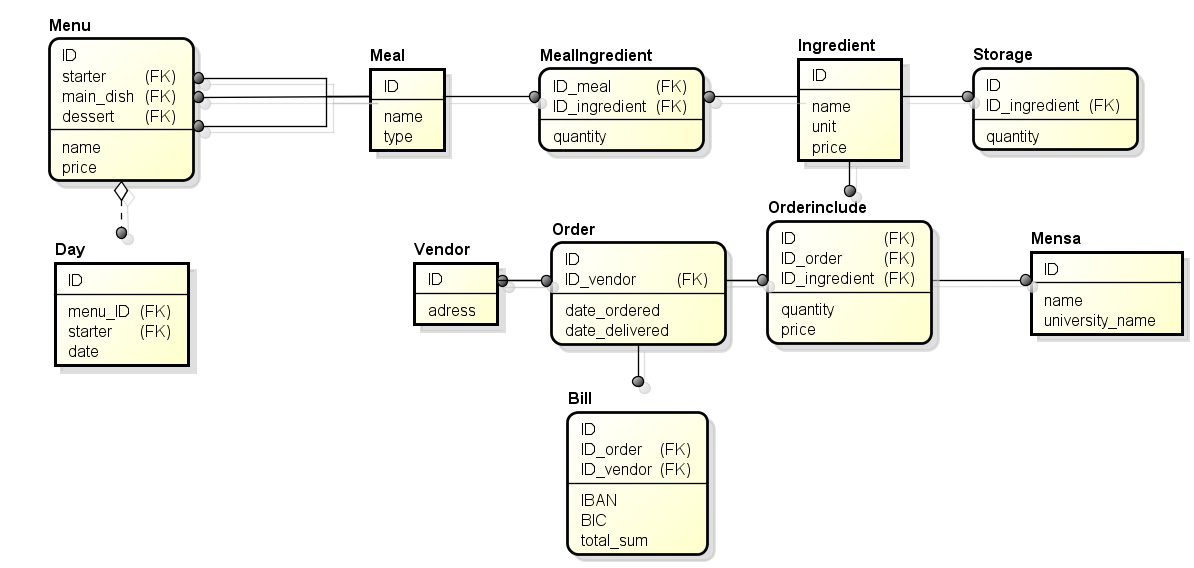
\includegraphics[width=1.0\textwidth]{images/er_vorlaeufig.png}
	\caption{The first try to make an working ER-Diagram with Astah}
	\label{fig:try1}
	\end{figure}
	
In figure \ref{fig:try2} our second database design can be seen. 
 \begin{figure}[here!]
	\centering
	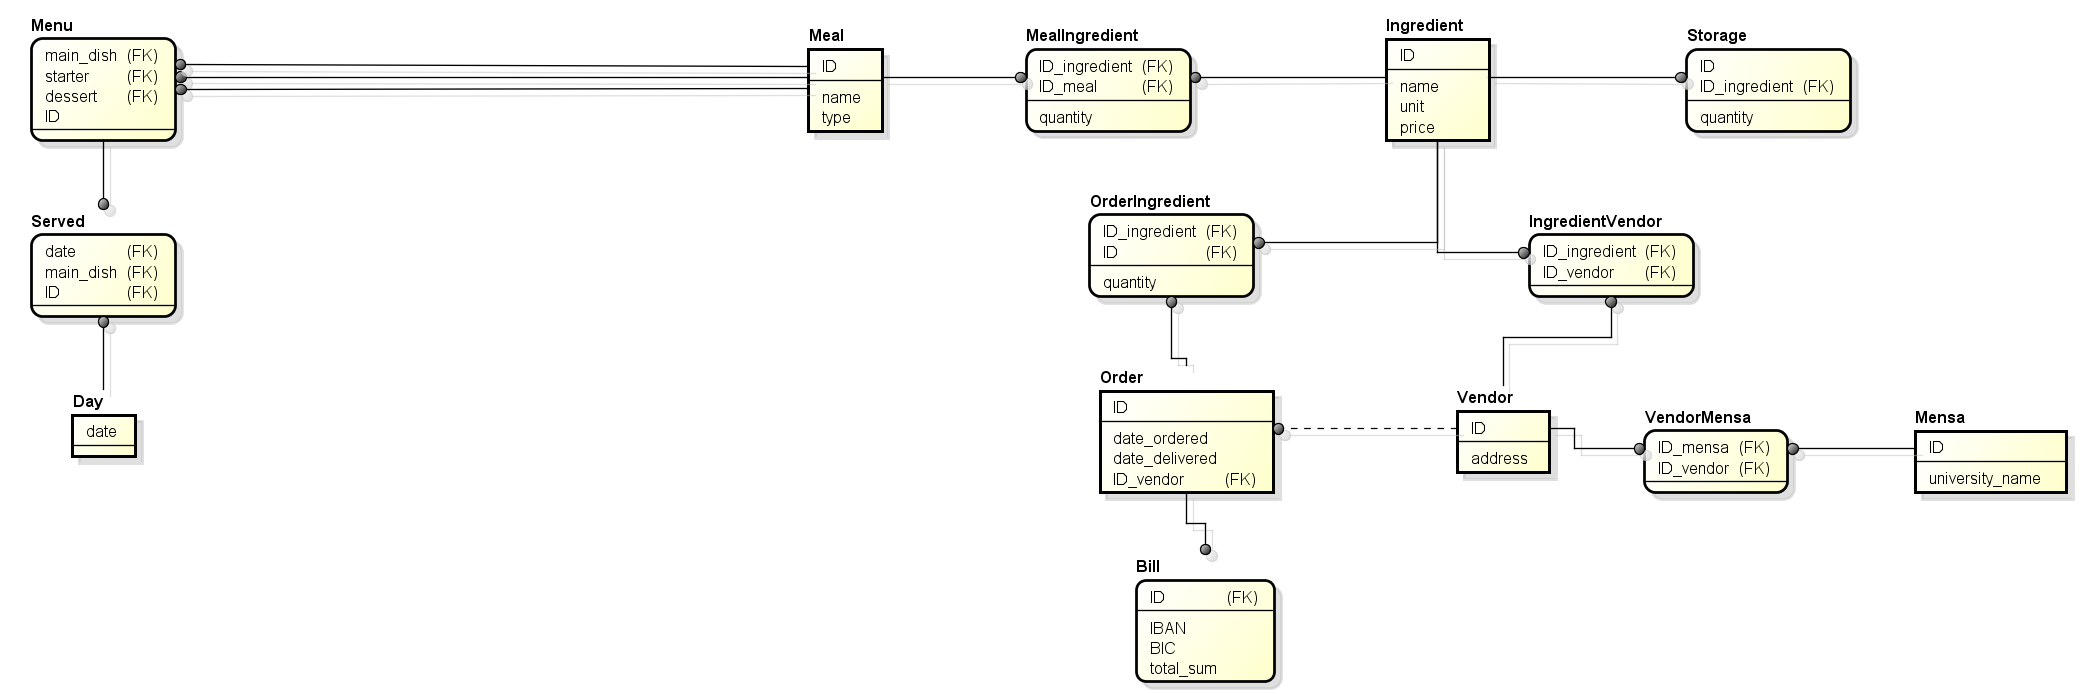
\includegraphics[width=1.0\textwidth]{images/neu.png}
	\caption{The second try to make an ER-Diagram using Astah}
	\label{fig:try2}
	\end{figure}	

After trying it for the second time to get the ER right, we decided that we will simply use the last \gls{er}-diagram and to change the little faults in the \gls{ddl} manually.
\FloatBarrier	
\subsubsection{\gls{ddl}}
Whenever using Astah, it is possible to export the \gls{er}-diagram into an \gls{sql} file. \\
Unfortunately this didn't work out, because we were not able to import the file which has been exported by Astah.
The syntax of the Order table was not right and we were not able to find a solution. The exported file will be in the disposal of this exercise. \\ \\
We then decided to simply code the \gls{ddl} by our selves, because we already know how to do so. It took us a little bit longer because there were some unnecessary faults, like a semicolon missing. We tried this using mysql at first and then we were migrating the code into an SQL-Language which could be understood by an Oracle Database as well.
In the end, we had an working \gls{ddl}.
\subsection{Setting up the Oracle DB}
First of all, we had to download the oracle VM from \cite{oraclevm}. Then it had to be imported into the VM-Ware. This process has been described under \cite{oraclevm2}.\\
\subsubsection{Importing the \gls{ddl}}
Adding the \gls{ddl}-file was quite easy:  \\
\texttt{@<filepath>} 
\subsubsection{Doing some Inserts}
We were doing an Insert in each Database. 
Doing inserts in Distributed Databases was exactly the same as if we'd done it on a normal one. 
\subsection{Setting up an Distributed Database}
\subsubsection{Fragmentation}
Oracle doesn't support vertical fragmentation. \\ Therefore we had to use a horizontal fragmentation, and nothing had to be changed.
\subsubsection{Creating a Link}
Creating a Link was surprisingly easy, as it can be seen in figure \ref{fig:endres}. \\
All we had to do was running: \\
\texttt{CREATE PUBLIC DATABASE LINK <remote-name> CONNECT TO <user> IDENTIFIED BY <password> USING '//<ip>:<port>/<service-name>';}
\subsubsection{Running some Selects}
Whenever a select statement should be done on a distributed database, the second database must be addressed using its link and an union:
\texttt{SELECT * FROM <table> UNION SELECT * FROM <table>@<remote-name>}
The output of one of these selects can be seen in figure \ref{fig:endres}

 \begin{figure}[here!]
	\centering
	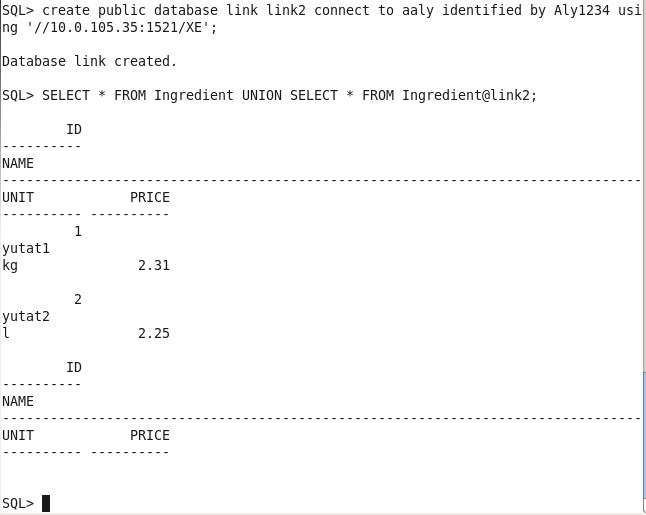
\includegraphics[width=1.0\textwidth]{images/endres.jpg}
	\caption{Setting up a link and making a select}
	\label{fig:endres}
	\end{figure}	
	
\newpage
\printglossaries
\listoffigures
\newpage
\begin{thebibliography}{56}

\bibitem{oraclevm}
   \textbf{Virtual Machine for the Oracle Communications Service 
Delivery Platform (SDP) Products}\newline
  \emph{http://www.oracle.com/technetwork/apps-tech/sdp-vm-2121008.html}
  \newline last used: 16.10.2014, 15:34


\bibitem{oraclevm2}
   \textbf{Oracle Communication 
Service Delivery Platform 
Environment}\newline
  \emph{http://download.oracle.com/otn/vm/sdp/SDP\_VM\_Instructions.pdf?AuthParam=1413466760\_7407137830244303d463cefcf991434a}
  \newline last used: 16.10.2014, 15:37




\end{thebibliography}

\end{document}

